\documentclass[border=10pt]{standalone}
\usepackage{tikz}
\usetikzlibrary{arrows.meta, shapes, calc}

\begin{document}

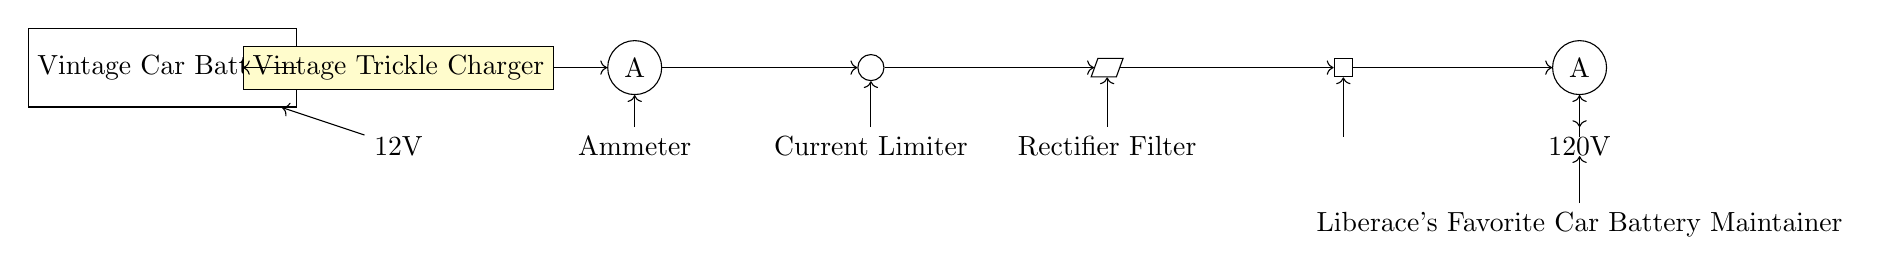
\begin{tikzpicture}[node distance=2cm, auto]
    \node (battery) [draw, rectangle, minimum width=2cm, minimum height=1cm] {Vintage Car Battery};
    \node (charger) [draw, rectangle, fill=yellow!20, right of=battery, node distance=3cm] {Vintage Trickle Charger};
    \node (ammeter) [draw, circle, right of=charger, node distance=3cm] {A};
    \node (current_limiter) [draw, circle, right of=ammeter, node distance=3cm] {};
    \node (rectifier) [draw, trapezium, trapezium left angle=70, trapezium right angle=110, right of=current_limiter, node distance=3cm] {};
    \node (filter) [draw, rectangle, right of=rectifier, node distance=3cm] {};
    \node (source) [draw, circle, right of=filter, node distance=3cm] {A};
    \node (text) [below of=source, node distance=1cm] {120V};
    \node (text2) [below of=charger, node distance=1cm] {12V};
    \node (text3) [below of=ammeter, node distance=1cm] {Ammeter};
    \node (text4) [below of=current_limiter, node distance=1cm] {Current Limiter};
    \node (text5) [below of=rectifier, node distance=1cm] {Rectifier Filter};
    \node (text6) [below of=filter, node distance=1cm] {};
    \node (text7) [below of=source, node distance=1cm] {};
    \node (text8) [below of=text7, node distance=1cm] {Liberace's Favorite Car Battery Maintainer};
    
    \draw [->] (battery) -- (charger);
    \draw [->] (charger) -- (ammeter);
    \draw [->] (ammeter) -- (current_limiter);
    \draw [->] (current_limiter) -- (rectifier);
    \draw [->] (rectifier) -- (filter);
    \draw [->] (filter) -- (source);
    
    \draw [->] (source) -- (text);
    \draw [->] (text2) -- (battery);
    \draw [->] (text3) -- (ammeter);
    \draw [->] (text4) -- (current_limiter);
    \draw [->] (text5) -- (rectifier);
    \draw [->] (text6) -- (filter);
    \draw [->] (text7) -- (source);
    \draw [->] (text8) -- (text7);
\end{tikzpicture}

\end{document}